\chapter{Isotropic energy probability densities in the laboratory frame}
\label{Sec:isotropic-lab}
The \xendl\ library supports several formats for energy probability densities
which are isotropic in the
laboratory frame.  These data are typically used for equilibrium
reactions and for fission neutrons.  Because the outgoing
distribution is isotropic, the probability density
$\pi(\Elab', \mulab   \mid E)$ in Eq.~(\ref{def_pi}) takes the form
\begin{equation}
  \pi(\Elab', \mulab   \mid E) = \pi_0(\Elab' \mid E).
 \label{isotropic-pi}
\end{equation}
Consequently, for the number-conserving
matrices only the $\ell = 0$ Legendre order,
\begin{equation}
   \Inum_{g,h,0} =
     \int_{\calE_g} dE \, \sigma ( E ) M(E) w(E) \widetilde \phi_0(E)
   \int_{\calE_h'} d\Elab' \, \pi_0(\Elab' \mid E)
 \label{InumI4-0}
\end{equation}
needs to be computed,
and Eq.~(\ref{Ien}) for the energy-preserving transfer matrix becomes
\begin{equation}
   \Ien_{g,h,0} =
     \int_{\calE_g} dE \, \sigma ( E ) M(E) w(E) \widetilde \phi_0(E) 
     \int_{\calE_h'} d\Elab' \, \pi_0(\Elab' \mid E) \Elab'.
 \label{IenI4-0}
\end{equation}

The data $\pi_0(\Elab' \mid E)$ may be given in \xendl\ either as
a table of values or as parameters in a function formula.
Because several of the function formulas for isotropic energy
probability densities are given in terms of incomplete gamma
functions, these are discussed first.  This is followed by a presentation
of the functional formulas for isotropic probability densities.  Then,
 the treatment of tables of~$\pi_0(\Elab' \mid E)$ for isotropic emission
 in the laboratory frame is discussed.  The section closes with
 the special treatment of the evaporation of delayed fission neutrons.

\section{Computational aspects of incomplete gamma functions}
Many
of the function formulas for $\pi_0(\Elab' \mid E)$ make use of the 
lower incomplete gamma function
\begin{equation}
  \gamma(\kappa, x) =
   \int_0^x dt\, t^{\kappa - 1} e^{-t}
  \label{def-gamma}
\end{equation}
with $\kappa > 0$.  The upper incomplete gamma
function is
\begin{equation}
  \Gamma(\kappa, x) =
   \int_x^\infty dt\, t^{\kappa - 1} e^{-t},
  \label{def-Gamma}
\end{equation}
and they are related by
$$
  \gamma(\kappa, x) + \Gamma(\kappa, x) = \Gamma(\kappa) =
  \int_0^\infty dt\, t^{\kappa - 1} e^{-t}.
$$
In order to reduce the difficulties of computer round-off,
the formula
$$
  \int_a^b dt\, t^{\kappa - 1} e^{-t} =
  \gamma( \kappa, b ) - \gamma( \kappa, a )
$$
is used when $0 \le a < b \le 1$, and
$$
  \int_a^b dt\, t^{\kappa - 1} e^{-t} =
  \Gamma( \kappa, a ) - \Gamma( \kappa, b )
$$
is used when $1 \le a < b$.  Either form may be used when
$a < 1 < b$.

Note that even though it is possible to write down
exact formulas for $\gamma(\kappa, x)$ when $\kappa$ is a
positive integer, it is better not to use them in the computations.
For example, it is true that
$$
  \gamma(2, x) = 1 - (1 + x)e^{-x}.
$$
For values of $x$ near zero, this formula involves subtracting
from 1 a number very close to 1 to get a result close to~$x^2/2$.
This is may lead to bad round-off errors in the computer arithmetic, 
and it is far better to
use the software for~$\gamma(2, x)$.

\section{Functional formulas for isotropic probability densities}
The functional formulas used in  \xendl\ for energy 
probability densities~$\pi_0(\Elab' \mid E)$ are the evaporation model,
the Maxwell model, the Watt model, and the Madland-Nix model.
These models are discussed in turn.  For all of these models the
energy of the outgoing particle is in the laboratory frame.

\subsection{Evaporation model}
For the evaporation model the formula is
\begin{equation}
  \pi_0(\Elab' \mid E) = C \Elab' \expon{- \frac{\Elab'}{\Theta(E)}}
 \label{evaporationF}
\end{equation}
with $0 \le \Elab' \le E - U$.  The value of $C$ in Eq.~(\ref{evaporationF})
is chosen so that
$$
  \int_0^{E - U} d\Elab' \, \pi_0(\Elab' \mid E) = 1.
$$
That is, 
$$
  C = \frac{1}{\Theta^2 \gamma(2, (E - U)/\Theta)}.
$$
The data consist of the energy of the reaction $U$ and pairs of
values $\{E, \Theta(E)\}$.  The 1-dimensional interpolation methods
of Section~\ref{Sec:1d-interp} are used to
determine the value of $\Theta$ for intermediate values of the 
energy $E$ of the incident particle.

According to the comment on incomplete gamma functions above,
for the calculation of $\Inum_{g,h,0}$ on an outgoing energy bin,
$E_0 \le \Elab' \le E_1$ the expression
$$
  \int_{E_0}^{E_1} d\Elab' \, \pi_0(\Elab' \mid E) =
   C\Theta^2[\gamma(2, E_1/\Theta) - \gamma(2, E_0/\Theta)]
$$
is used when $E_0 \le \Theta$, and
$$
  \int_{E_0}^{E_1} d\Elab' \, \pi_0(\Elab' \mid E) =
   C\Theta^2[\Gamma(2, E_0/\Theta) - \Gamma(2, E_1/\Theta)]
$$
is used when $E_0 > \Theta$.  Analogously, for the
calculation of $\Ien_{g,h,0}$
$$
  \int_{E_0}^{E_1} d\Elab' \, \Elab' \pi_0(\Elab' \mid E) =
   C\Theta^3[\gamma(3, E_1/\Theta) - \gamma(3, E_0/ \Theta)]
$$
is used when $E_0 \le \Theta$, and
$$
  \int_{E_0}^{E_1} d\Elab' \, \Elab' \pi_0(\Elab'  \mid E) =
   C\Theta^3[\Gamma(3, E_0/\Theta) - \Gamma(3, E_1/\Theta)]
$$
is used otherwise.

\subsubsection{Input file data for the evaporation model}
The process identifier in Section~\ref{data-model} is\\
  \Input{Process: evaporation spectrum}{}\\
These data are always in the laboratory frame,\\
  \Input{Product Frame: lab}{}

One item of model-dependent data in Section~\ref{model-info}
is the value of $U$ used in defining the range of outgoing
energies $E$ in Eq.~(\ref{evaporationF}), and it is given by\\
  \Input{U:}{$U$}\\
The other input data are the values of $\Theta(E)$ in
Eq.~(\ref{evaporationF}) depending on the incident energy~$E$.  
All of these energies, $U$, $E$, and $\Theta(E)$, must be in the same
units as the energy bins in Sections~\ref{Ein-bins} and~\ref{Eout-bins}.
The format for these data is\\
  \Input{Theta: n = $n$}{}\\
  \Input{Interpolation:}{interpolation flag}\\
with $n$ pairs of entries $\{E, \Theta(E)\}$.  
The interpolation flag is one of those for simple lists as in 
Section~\ref{interp-flags-list}.
For example, in units of MeV one may have\\
  \Input{U: 11.6890}{}\\
  \Input{Theta: n = 2}{}\\
  \Input{Interpolation: lin-lin}{}\\
  \Input{ 12.0 1.04135}{}\\
  \Input{ 20.0 1.04135}{}

\subsection{Maxwell model}
The formula for the Maxwell is
\begin{equation}
  \pi_0(\Elab'  \mid E) = C \sqrt{\Elab' } \, \expon{- \frac{\Elab' }{\Theta(E)}}
 \label{MaxwellF}
\end{equation}
for $0 \le \Elab'  \le E - U$.  This model is often used for fission neutrons.
The value of $C$ in Eq.~(\ref{MaxwellF}) is given by
$$
  C = \frac{1}{\Theta^{3/2} \gamma(3/2, (E - U)/\Theta)}.
$$
Because of round-off problems with small values of $x$,
it is unwise to use the mathematically equivalent formula
$$
  \gamma(3/2, x) =
  \frac{\sqrt{\pi}}{2}\, \erf{\sqrt{x}} - \sqrt{x}\,e^{-x}.
$$
The data consist of the energy of the reaction $U$ and pairs of
values $\{E, \Theta(E)\}$.  The parameter $\Theta$ is interpolated
by the methods of Section~\ref{Sec:1d-interp} to obtain intermediate values. 

Depending on the value of $E_0/\Theta$,
the calculation of $\Inum_{g,h,0}$ on an outgoing energy bin
$E_0 \le \Elab'  \le E_1$ uses the expression
$$
  \int_{E_0}^{E_1} d\Elab'  \, \pi_0(\Elab'  \mid E) =
   C\Theta^{3/2}[\gamma({3/2}, E_1/\Theta) - \gamma({3/2}, E_0/\Theta)]
$$
or
$$
  \int_{E_0}^{E_1} d\Elab'  \, \pi_0(\Elab'  \mid E) =
   C\Theta^{3/2}[\Gamma({3/2}, E_0/\Theta) - \Gamma({3/2}, E_1/\Theta)].
$$
Analogously, the calculation of $\Ien_{g,h,0}$ uses either
$$
  \int_{E_0}^{E_1} d\Elab'  \, \Elab' \pi_0(\Elab'  \mid E) =
   C\Theta^{5/2}[\gamma({5/2}, E_1/\Theta) - \gamma({5/2}, E_0/\Theta)]
$$
or
$$
  \int_{E_0}^{E_1} d\Elab'  \, \Elab' \pi_0(\Elab'  \mid E) =
   C\Theta^{5/2}[\Gamma({5/2}, E_0/\Theta) - \Gamma({5/2}, E_1/\Theta)].
$$

\subsubsection{Input file data for the Maxwell model}
The process identifier in Section~\ref{data-model} is\\
  \Input{Process: Maxwell spectrum}{}\\
Again, this data is in the laboratory frame,\\
  \Input{Product Frame: lab}{}

One item of model-dependent data in Section~\ref{model-info}
is the value of $U$ used in defining the range of outgoing
energies $E$ in Eq.~(\ref{MaxwellF}), and it is given by\\
  \Input{U:}{$U$}\\
The other input data are the values of $\Theta(E)$ in
Eq.~(\ref{MaxwellF}) depending on the incident energy~$E$.  
These energies, $U$, $E$, and $\Theta(E)$, must all be in the same
units as the energy bins in Sections~\ref{Ein-bins} and~\ref{Eout-bins}.
The format for such data is\\
  \Input{Theta: n = $n$}{}\\
  \Input{Interpolation:}{interpolation flag}\\
with $n$ pairs of entries $\{E, \Theta(E)\}$.  
The interpolation flag is one of those for simple lists as in 
Section~\ref{interp-flags-list}.
For example, in units of MeV one may have\\
  \Input{U: -20}{}\\
  \Input{Theta: n = 2}{}\\
  \Input{Interpolation: lin-lin}{}\\
  \Input{ 1.0e-11  1.28}{}\\
  \Input{ 20.0  1.28}{}

\subsection{Watt model}
Another model sometimes used for fission neutrons in \xendl\ is the Watt
formula
\begin{equation}
  \pi_0(\Elab'  \mid E) = C \sinh{\sqrt{b\Elab' }}\, \expon{- \frac{\Elab' }{a}}
 \label{WattF}
\end{equation}
for $0 \le \Elab'  \le E - U$.
The value of $C$ in Eq.~(\ref{WattF})
is given by
$$
  \frac{1}{C} =
  \frac{az\sqrt{\pi}}{2}\, \expon{z^2}
  \left(
    \erf{y - z} - \erf{y + z}
  \right) -
  a \expon{-y^2} \sinh{\sqrt{b(E - U)}}
$$
with $y = \sqrt{(E - U)/a}$ and $z = \sqrt{ab /4}$.
The data consist of the energy of the reaction $U$ and pairs of
values $\{E, a(E)\}$ and $\{E, b(E)\}$.  For intermediate incident
energies $E$, the parameters $b$ and~$a$ are interpolated by
the methods of Section~\ref{Sec:1d-interp}.

\subsubsection{Input file data for the Watt model}
The process identifier in Section~\ref{data-model} is\\
  \Input{Process: Watt spectrum}{}\\
This data is in the laboratory frame,\\
  \Input{Product Frame: lab}{}

One item of model-dependent data in Section~\ref{model-info}
is the value of $U$ used in defining the range of outgoing
energies $E$ in Eq.~(\ref{WattF}), and it is given by\\
  \Input{U:}{$U$}\\
The other input data are the values of $a(E)$ and $b(E)$ in
Eq.~(\ref{WattF}).  
The energies, $U$, $E$, and $a(E)$, must be in the same
units as the energy bins in Sections~\ref{Ein-bins} and~\ref{Eout-bins},
and the units for $b(E)$ are the reciprocal of these units.
The format for these data is\\
  \Input{a: n = $n$}{}\\
  \Input{Interpolation:}{interpolation flag}\\
with $n$ pairs of entries $\{E, a(E)\}$ and\\
  \Input{b: n = $n$}{}\\
  \Input{Interpolation:}{interpolation flag}\\
with $n$ pairs of entries $\{E, b(E)\}$.
The interpolation flags for $a$ and $b$ are those for simple lists as in 
Section~\ref{interp-flags-list}.
For example, with energies in MeV  one may have\\
  \Input{U: -10}{}\\
  \Input{a: n = 11}{}\\
  \Input{Interpolation: lin-lin}{}\\
  \Input{ 1.000000e-11    9.770000e-01}{}\\
  \Input{ 1.500000e+00   9.770000e-01}{}\\
  \Input{}{ $\cdots$}\\
     \Input{ 3.000000e+01 1.060000e+00}{}\\
  \Input{b: n = 11}{}\\
  \Input{Interpolation: lin-lin}{}\\
  \Input{ 1.000000e-11    2.546000e+00}{}\\
  \Input{ 1.500000e+00   2.546000e+00}{}\\
  \Input{}{ $\cdots$}\\
     \Input{ 3.000000e+01 2.620000e+00}{}

\subsection{Madland-Nix model}\label{Sec:Madland}

The Madland-Nix model~\cite{Madland} for prompt fission neutrons uses 
the formula
\begin{equation}
  \pi_0(\Elab'  \mid E) = \frac{C}{2}\, [g(\Elab' , E_{FL}) + g(\Elab' , E_{FH})]
 \label{Madland-NixF}
\end{equation}
for
\begin{equation}
 0 \le \Elab' \le \texttt{maxEout},
 \label{Madland-Nix-E-range}
\end{equation}
where \texttt{maxEout} is one of the input parameters.
Note that the range of outgoing energies Eq.~(\ref{Madland-Nix-E-range})
is independent of the incident energy.
In fact, the \ENDF\ manual~\cite{ENDFB} gives no way for the data to specify the
maximum outgoing energy for the Madland-Nix model. 

In Eq.~(\ref{Madland-NixF}) $E_{FL}$ is the average kinetic energy of the light fission
fragments, and $E_{FH}$ is the average kinetic energy of the heavy fission
fragments.  The function $g(\Elab' , E_F)$ in Eq.~(\ref{Madland-NixF}) is given in terms
of the parameters $T_m$ and
\begin{equation}
   u_1 = \frac{(\sqrt{\Elab' } - \sqrt{E_F})^2}{T_m}, \quad
   u_2 = \frac{(\sqrt{\Elab' } + \sqrt{E_F})^2}{T_m}
 \label{Madland-Nixu}
\end{equation}
by the formula
\begin{equation}
   g(\Elab' , E_F) = \frac{1}{3\sqrt{E_F T_m}}
   \left[
     u_2^{3/2}E_1(u_2) - u_1^{3/2}E_1(u_1) -
     \Gamma(3/2, u_2) + \Gamma(3/2, u_1)
   \right],
 \label{Madland-Nixg}
\end{equation}
where $E_1$ denotes the exponential integral
$$
  E_1(x) = \int_x^\infty dt\, \frac{1}{t}e^{-t}.
$$
It is clear from the definitions that
$$
  E_1(x) = \Gamma(0, x),
$$
but software to compute $\Gamma(\kappa, x)$ generally requires
that $\kappa$ be positive.
The data for the Madland-Nix model contains the average energies
$E_{FL}$ and $E_{FH}$ as well as pairs of values $\{E, T_m(E)\}$.
The interpolation rule for $T_m$ is also given.

If the range of outgoing energies is taken to be $0 \le \Elab'  < \infty$ 
in Eq.~(\ref{Madland-NixF}), then $C = 1$.  For other ranges of $\Elab' $
and for computation of $\Inum_{g,h,0}$, it follows from Eq.~(\ref{Madland-Nixg})
that it is necessary to compute integrals
\begin{equation}
 \calG_i( a, b ) =  \int_a^b d\Elab'  \, u_i^{3/2}E_1(u_i)
 \label{Madland-Nix-u-integral}
\end{equation}
and
\begin{equation}
 \calH_i( a, b ) =   \int_a^b d\Elab'  \, \Gamma(3/2, u_i)
 \label{Madland-Nix-Gamma-integral}
\end{equation}
with $i = 1$, 2.

The values of the integrals Eqs.~(\ref{Madland-Nix-u-integral})
and~(\ref{Madland-Nix-Gamma-integral}) are conveniently expressed
in terms of the parameters
\begin{equation}
  \alpha = \sqrt{T_m}, \quad
  \beta = \sqrt{E_F},
 \label{Madland-Nix-alpha-beta}
\end{equation}
\begin{equation}
  A = \frac{(\sqrt{a} + \beta)^2}{\alpha^2}, \quad
  B = \frac{(\sqrt{b} + \beta)^2}{\alpha^2},
 \label{Madland-Nix-A-B}
\end{equation}
and
\begin{equation}
  A' = \frac{( \beta - \sqrt{a})^2}{\alpha^2}, \quad
  B' = \frac{(\sqrt{b} - \beta)^2}{\alpha^2}.
 \label{Madland-Nix-A-B-prime}
\end{equation}

One might think it sufficient to calculate
$$
  \calG_i( 0, b )  \quad \text{and} \quad
  \calH_i( 0, b ) 
$$
in Eqs.~(\ref{Madland-Nix-u-integral}) and~(\ref{Madland-Nix-Gamma-integral})
and to use
\begin{equation*}
 \begin{split}
   \calG_i( a, b ) &= \calG_i( 0, b ) - \calG_i( 0, a ), \\
   \calH_i( a, b ) &= \calH_i( 0, b ) - \calH_i( 0, a )
 \end{split}
\end{equation*}
for $i = 1$, 2.  In fact, this approach is suitable only for $i = 2$.
The reason for the difficulty is seen from Eqs.~(\ref{Madland-Nixu})
and~(\ref{Madland-Nix-alpha-beta}), in that
\begin{equation}
  u_1^{3/2} = \begin{cases}
    (\beta - \sqrt{\Elab' })^3 / \alpha^3  \quad &\text{for $0 \le \Elab'  \le \beta^2$}, \\
    (\sqrt{\Elab' } - \beta)^3 / \alpha^3 \quad &\text{for $\Elab'  > \beta^2$}.
    \end{cases}
 \label{Madland-Nix-u1}
\end{equation}

Consequently, the integrals used to compute $\calG_i( a, b )$
and~$\calH_i( a, b )$ in Eqs.~(\ref{Madland-Nix-u-integral}) 
and (\ref{Madland-Nix-Gamma-integral}) are evaluated as
\begin{equation}
  \calG_1( a, \beta^2 ) = 
    \frac{\alpha \beta}{2} \, \gamma \left( 2, A' \right)
       -\frac{2 \alpha^2}{5} \, \gamma \left( \frac{5}{2}, A' \right) +
       \left[
          \frac{2 \alpha \sqrt{A'}}{5} - \frac{\beta}{2}
        \right] \alpha {A'}^2 E_1( A' )
       \quad \text{for $0 \le a < \beta^2$},
\label{Madland-Nix-G1a}
\end{equation}
\begin{equation}
  \calG_1( \beta^2, b ) = 
    \frac{\alpha \beta}{2} \, \gamma \left( 2, B' \right)
       + \frac{2 \alpha^2}{5} \, \gamma \left( \frac{5}{2}, B' \right) +
       \left[
          \frac{\beta}{2} + \frac{2 \alpha \sqrt{B'}}{5}
        \right] \alpha {B'}^2 E_1( B' )
       \quad \text{for $b > \beta^2$},
 \label{Madland-Nix-G1b}
\end{equation}
\begin{equation}
 \begin{split}
  \calG_2( 0, b )  = &
    \frac{2 \alpha^2}{5} \, \gamma \left( \frac{5}{2}, B \right) -
    \frac{\alpha \beta}{2} \, \gamma \left( 2, B \right) -
    \frac{\beta^5}{10 \alpha^3} \,e^{-B} + {}\\
      & \left[
        \frac{2 \alpha^2}{5} B^{5/2} - \frac{\alpha \beta}{2} {B}^2 +
          \frac{ \beta^5}{10 \alpha^3} \right]  E_1( B) - C_1
       \quad \text{for $b \ge 0$},
 \end{split}
\label{Madland-Nix-G2}
\end{equation}
\begin{equation}
  \calH_1(a, \beta^2) = 2 \alpha \beta \, \gamma \left( 2, A' \right) -
  \alpha^2 \, \gamma \left( \frac{5}{2}, A' \right) +
     (\beta^2 - a) \, \Gamma\left( \frac{3}{2}, A' \right)
     \quad \text{for $0 \le a < \beta^2$},
\label{Madland-Nix-H1a}
\end{equation}
\begin{equation}
  \calH_1(\beta^2, b) = 2 \alpha \beta \, \gamma \left( 2, B' \right) +
     \alpha^2 \, \gamma \left( \frac{5}{2}, B' \right) +
     (b - \beta^2) \, \Gamma\left( \frac{3}{2}, B' \right)
     \quad \text{for $b \ge \beta^2$},
\label{Madland-Nix-H1b}
\end{equation}
and
\begin{equation}
   \calH_2(0, b) = \alpha^2 \, \gamma \left( \frac{5}{2}, B \right) -
     2 \alpha\beta \, \gamma \left( 2, B \right) +
     \beta^2 \, \gamma \left( \frac{3}{2}, B \right) +
     b \, \Gamma \left( \frac{3}{2}, B \right) - C_2
     \quad \text{for $b > 0$}.
\label{Madland-Nix-H2}
\end{equation}
In the relations for $\calG_2(0, b)$ and $\calH_2(0, b)$ above, $C_1$
and~$C_2$ are constants of integration.

\begin{figure}
% domain of integration for the Madland-Nix model
\begin{center}
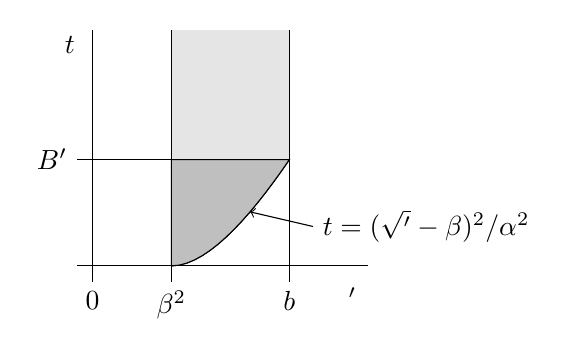
\begin{tikzpicture}
% the u_1(E) curve
\draw( 1.0 , 0.0 ) --
( 1.1 , 0.00952921463879 ) --
( 1.2 , 0.0364390799173 ) --
( 1.3 , 0.0785965992069 ) --
( 1.4 , 0.134272347041 ) --
( 1.5 , 0.202041028867 ) --
( 1.6 , 0.280711487461 ) --
( 1.7 , 0.369276151676 ) --
( 1.8 , 0.466873708001 ) --
( 1.9 , 0.572760998328 ) --
( 2.0 , 0.686291501015 ) --
( 2.1 , 0.806898603048 ) --
( 2.2 , 0.934082420647 ) --
( 2.3 , 1.06739928952 ) --
( 2.4 , 1.20645329214 ) --
( 2.5 , 1.35088935933 );
% integration regions
\filldraw[fill = gray!50]
( 1.0 , 0.0 ) --
( 1.1 , 0.00952921463879 ) --
( 1.2 , 0.0364390799173 ) --
( 1.3 , 0.0785965992069 ) --
( 1.4 , 0.134272347041 ) --
( 1.5 , 0.202041028867 ) --
( 1.6 , 0.280711487461 ) --
( 1.7 , 0.369276151676 ) --
( 1.8 , 0.466873708001 ) --
( 1.9 , 0.572760998328 ) --
( 2.0 , 0.686291501015 ) --
( 2.1 , 0.806898603048 ) --
( 2.2 , 0.934082420647 ) --
( 2.3 , 1.06739928952 ) --
( 2.4 , 1.20645329214 ) --
( 2.5 , 1.35088935933 ) --
(1, 1.35088935933 ) -- cycle;
\fill[ gray!20] ( 2.5 , 1.35088935933 ) --
(2.5, 3) -- (1, 3) --
( 1 , 1.35088935933 ) -- cycle;
% the axes and quadrature strip
 \draw(-0.2, 0) -- (3.5, 0);
 \draw(0, -0.2) -- (0, 3);
 \draw(-0.2, 1.35088935933) -- (2.5, 1.35088935933);
 \draw(1, -0.2) -- (1, 3);
 \draw(2.5, -0.2) -- (2.5, 3);
% labels
  \node [below] at (0, -0.2){0};
  \node [below] at (1, -0.2){$\beta^2$};
  \node [below] at (2.5, -0.2){$b$};
  \node [below] at (3.3, -0.15){$\Elab'$};
  \node [left] at (-0.2, 1.35){$B'$};
  \node [left] at (-0.1, 2.8){$t$};
  %legend
  \draw [<-] ( 2.0 , 0.686291501015 ) -- (2.8, 0.5);
  \node [right] at (2.8, 0.5) {$ t = (\sqrt{\Elab'} - \beta)^2/\alpha^2$};
\end{tikzpicture}
\caption{Domain of integration for $\calG_1( \beta^2, b )$ with $b > \beta^2$
in the Madland-Nix model}
\label{Fig:Madland-Nix}
\end{center} 

\end{figure}

In order to illustrate how the above integration formulas may be 
derived, consider the case of Eq.~(\ref{Madland-Nix-G1b})
for $\calG_1( \beta^2, b )$ defined in 
Eq.~(\ref{Madland-Nix-u-integral}) with $u_1$ as in
Eq.~(\ref{Madland-Nix-u1}) and with~$b > \beta^2$.  Substitution
of the definition of the exponential integral~$E_1$ gives the double
integral
$$
   \calG_1( \beta^2, b ) = \int_{\beta^2}^b d\Elab'  \,
      u_1^{3/2} \int_{u_1}^\infty dt \, \frac{1}{t} \, e^{-t}.
$$
The region of integration for this integral is the union of the
two shaded domains in Figure~\ref{Fig:Madland-Nix}.
The integral over the darker shaded region of Figure~\ref{Fig:Madland-Nix} is
$$
  J_{11} = \int_{\beta^2}^b d\Elab'  \, u_1^{3/2}\int_{u_1}^{B'} dt\, \frac { e^{-t}}{t}.
$$
Reversal of the order of integration transforms this integral to
$$
  J_{11} = \int_0^{B'} dt\, \frac{1}{t} \,e^{-t}
    \int_{\beta^2}^{(\alpha\sqrt{t} + \beta)^2}
       d\Elab' \, u_1^{3/2}.
$$
Under the substitution
\begin{equation*}
  \Elab'  = (\alpha \sqrt{u_1} + \beta)^2,
%  \label{u_for_E}
\end{equation*}
the inner integral takes the form
$$
  \int_{\beta^2}^{(\alpha\sqrt{t} + \beta)^2}
       d\Elab' \, u_1^{3/2} =
   \int_0^t du_1 \, u_1^{3/2}\left( 
       \alpha^2 + \frac{\alpha\beta}{\sqrt{u_1}} 
  \right) =
    \frac{2\alpha^2}{5}t^{5/2} + \frac{\alpha\beta}{2}t^2.
$$
Thus, it follows that the integral over the dark shaded region in
Figure~\ref{Fig:Madland-Nix} is
\begin{equation*}
  J_{11} = 
    \frac{2\alpha^2}{5} \, \gamma(5/2, B') + \frac{ \alpha\beta}{2} \, \gamma(2, B').
%  \label{intJ11}
\end{equation*}
This relation gives the first two terms on the right-hand side
of Eq.~(\ref{Madland-Nix-G1b}).

The other terms on the right-hand side of Eq.~(\ref{Madland-Nix-G1b})
result from evaluation of the integral over the light shaded region in
Figure~\ref{Fig:Madland-Nix},
$$
J_{12} = \int_{\beta^2}^b d\Elab'  \, u_1^{3/2} \int_{B'}^\infty dt\, \frac {e^{-t}}{t}
 = \int_{B'}^\infty dt\, \frac{1}{t} \, e^{-t}
    \int_{\beta^2}^{b}
       d\Elab' \, u_1^{3/2}.
$$  

\subsubsection{Input file data for the Madland-Nix model}
The process identifier in Section~\ref{data-model} is\\
  \Input{Process: Madland-Nix spectrum}{}\\
This data is in the laboratory frame,\\
  \Input{Product Frame: lab}{}

The model-dependent data in Section~\ref{model-info}
contains values of $E_{FL}$, the average kinetic energy of the
light fission fragment and $E_{FH}$, the average kinetic energy of the
heavy fission fragment.  These parameters are given by\\
  \Input{EFL:}{$E_{FL}$}\\
  \Input{EFH:}{$E_{FH}$}\\
The user must also specify a maximum outgoing energy 
\texttt{maxEout} for use in Eq.~(\ref{Madland-Nix-E-range}).
 
The other input data are the values of $T_m$ as a function of
incident energy in
Eq.~(\ref{Madland-NixF}).  The format for these data is\\
  \Input{TM: n = $n$}{}\\
  \Input{Interpolation:}{interpolation flag}\\
with $n$ pairs of entries $\{E, T_m(E)\}$.  
The interpolation flag is one of those for simple lists as in 
Section~\ref{interp-flags-list}.
The energies, $E_{FL}$, $E_{FH}$, $E$, and $T_m(E)$, must be in the same
units as the energy bins in Sections~\ref{Ein-bins} and~\ref{Eout-bins}.
For example, in MeV units one may have\\
  \Input{EFL: 1.029979}{}\\
  \Input{EFH: 0.5467297}{}\\
  \Input{maxEout: 60}{}\\
  \Input{TM: n = 38}{}\\
  \Input{Interpolation: lin-lin}{}\\
  \Input{ 1.0000000e-11   1.0920640e+00}{}\\
  \Input{ 5.0000010e-01  1.1014830e+00}{}\\
  \Input{}{ $\cdots$}\\
  \Input{ 2.0000000e+01  1.1292690e+00}{}

\section{Energy probability density tables}\label{Sec:isotropicTables}
Another form of isotropic probability density data $\pi_0(\Elab'  \mid E)$
Eq.~(\ref{isotropic-pi}) in \xendl\ is in the form of tables.  The computation
of transfer matrices for such data given in the laboratory frame is
discussed here.  For data in the center-of-mass frame, this is a
special case of Legendre expansions discussed in Section~\ref{Ch:Legendre-cm}
with Legendre order zero.
For given
incident energies $E_i$, the data consist of pairs 
$\{E_{k,j}', \pi_0(E_{k,j}' \mid E_k)\}$ as in Eq.~(\ref{EPtable}).
For such tabular data,
computation of the integrals $\Inum_{g,h,0}$ in Eq.~(\ref{InumI4-0})
and $\Ien_{g,h,0}$ in Eq.~(\ref{IenI4-0}) depends on the type
of interpolation used between
different incident energies.
The effects of the unit-base map Eq.~(\ref{unit-base-map}) are
discussed here.  The considerations are the same, whether the
unit-base map is used alone or as a component of interpolation
by cumulative points.

After the unit-base transformation Eq.~(\ref{unit-base-map})
the integrals Eqs.~(\ref{InumI4-0}) and~(\ref{IenI4-0}) take the form
\begin{equation}
   \Inum_{g,h,0} =
     \int_{\calE_g} dE \, \sigma ( E ) M(E) w(E) \widetilde \phi_0(E) 
   \int_{\widehat\calE_h'} d\widehat \Elab'  \,
     \widehat\pi_0(\widehat \Elab'   \mid E)
 \label{InumhatI4-0}
\end{equation}
and
\begin{equation}
   \Ien_{g,h,0} =
     \int_{\calE_g} dE \, \sigma ( E ) M(E) w(E) \widetilde \phi_0(E) 
   \int_{\widehat\calE_h'} d\widehat \Elab'   \,
     \widehat\pi_0(\widehat \Elab'   \mid E) \Elab'  .
 \label{IenhatI4-0}
\end{equation}
In these intergrals $\widehat\calE_h'$ denotes result of mapping the 
outgoing energy bin $\calE_h'$ with the transformation Eq.~(\ref{unit-base-map}).
Furthermore, $\Elab'  $ in Eq.~(\ref{IenhatI4-0}) is to be obtained from $\widehat \Elab'  $
using the inverse unit-base mapping Eq.~(\ref{unitbaseInvert}).

\begin{figure}
% domain of integration for energy probability density tables
\begin{center}
\begin{tikzpicture}
% the axes and quadrature strip
% the axes
  \draw(-0.2,0) -- (3.8, 0);
  \draw(0,-0.2) -- (0, 4);
  \node [below] at (3.8, -0.15){$E$};
  \node [left] at (-0.1, 2.8){$E'$};
% the E' lines
  \draw(1,-0.2) -- (1, 1);
  \draw(3,-0.2) -- (3, 4);
% integration box
  \draw(0.8, 0.8) -- (0.8, 1.8) --
  (2.4, 1.8) --
  (2.4, 0.8) -- cycle;
% labels
  \node [below] at (1, -0.2){$E_{k-1}$};
  \node [below]  at (3, -0.2){$E_{k}$};
  \node [left] at (0.8, 1.2){$\calE_h'$};
  \node [above] at (1.15, 1.8){$\calE_g$};
% the curves
  \draw(1,0.25) -- (3,1);
  \draw (1, 0.5) -- (3, 2);
  \draw (1, 1) -- (3, 4);
% integration region
\filldraw[fill = gray!50]
  (2.4, 0.8) -- (2.4, 1.55) -- (1.4, 0.8) -- cycle;
%%% the mapped picture
% the axes
  \draw(5.9,0) -- (9.8, 0);
  \draw(6,-0.2) -- (6, 4);
  \node [below] at(9.8, -0.15){$E$};
  \node [left] at(5.9, 3.8){$\widehat E'$};
  \draw(5.8,3) -- (6, 3);
  \node [left] at(5.8, 3){$1$};
  \node [left] at(5.8, 0){$0$};
  \draw(5.8,0.75) -- (6, 0.75);
  \node [left] at (5.8, 0.75){$\widehat E_{j-1}'$};
  \draw(5.8,1.5) -- (6, 1.5);
  \node [left] at (5.8, 1.5){$\widehat E_{j}'$};
% the E' lines
  \draw(7,-0.2) -- (7, 3);
  \draw(9,-0.2) -- (9, 3);
% the Ehat lines
  \draw(7, 0.75) -- (9, 0.75);
  \draw(7, 1.5) -- (9, 1.5);
  \draw(7, 3) -- (9, 3);
% integration box
  \draw(6.8, 3.4286) -- (6.8, 7.7143);
  \draw(8.4, 0.7743) -- (8.4, 1.74194);
% Eout: 0.8
\draw(6.8, 3.42857) --
(6.96, 2.55319) --
(7.12, 2.0339) --
(7.28, 1.69014) --
(7.44, 1.44578) --
(7.6, 1.26316) --
(7.76, 1.1215) --
(7.92, 1.0084) --
(8.08, 0.916031) --
(8.24, 0.839161) --
(8.4, 0.774194);
% Eout: 1.8
\draw(6.8, 7.71429) --
(6.96, 5.74468) --
(7.12, 4.57627) --
(7.28, 3.80282) --
(7.44, 3.25301) --
(7.6, 2.84211) --
(7.76, 2.52336) --
(7.92, 2.26891) --
(8.08, 2.06107) --
(8.24, 1.88811) --
(8.4, 1.74194);
% integration region
\filldraw[fill = gray!50]
  (8.4, 0.774194) -- (8.4, 1.5) --
  (7.4045, 1.5) -- (7.44, 1.44578) --
(7.6, 1.26316) --
(7.76, 1.1215) --
(7.92, 1.0084) --
(8.08, 0.916031) --
(8.24, 0.839161) -- cycle;
% labels
  \node [below] at (7, -0.2){$E_{k-1}$};
  \node [below] at (9, -0.2){$E_k$};
  \node [left] at (6.8, 5.2){$\widehat \calE_h'$};
  \node [right] at (7.3, 4){$\calE_g$};
%legend
\draw [{<[scale=2, length=3, width=3]}-] (2.75, 0.9063) -- (3.5, 5.5);
\node [left] at (3.5, 5.5) {$\widehat E' = \widehat E_j'$};
\draw [{<[scale=2, length=3, width=3]}-] (2.5, 1.625) -- (2.7, 4.5);
\node [left] at (2.7, 4.5) {$\widehat E' = \widehat E_{j-1}'$};
\end{tikzpicture}
\caption{Domains of integration for tabulated probability densities, laboratory
frame on the left and unit base on the right}
\label{Fig:unit-base-region}
\end{center} 

\end{figure}

Figure~\ref{Fig:unit-base-region} illustrates the effect of
the unit-base map Eq.~(\ref{unit-base-map}).   
For incident energies $E = E_{k-1}$ and~$E = E_k$,  
1-dimensional interpolation is used
to produce data at a common set of unit-base outgoing energies
$\{\widehat E_j'\}$. In the left-hand
portion of Figure~\ref{Fig:unit-base-region}, suppose that
probability densities $\pi_0(\Elab'   \mid E)$ are given at incident energies
$E = E_{k-1}$ and~$E = E_k$ and at unit-base outgoing energies
 $\widehat E_{j-1}'$ and $\widehat E_j'$.  
Then for this set of data, the range of 
integration over $E$ in Eqs.~(\ref{InumhatI4-0}) or (\ref{IenhatI4-0}) requires
both that $E_{k-1} < E < E_k$ and that $E$ be in the bin~$\calE_g$.  The
outgoing energy~$\Elab'  $ is required to be in the bin~$\calE_h'$ and to satisfy
the constraint $\widehat E_{j-1}' < \widehat \Elab'   < \widehat E_j'$.

 The right-hand portion of Figure~\ref{Fig:unit-base-region}
shows a rectangle with vertices at $E = E_{k-1}$ and~$E = E_k$
and at $\widehat \Elab'   = \widehat E_{j-1}'$ and~$\widehat \Elab'   = \widehat E_j'$,
and data values $\widehat\pi_\ell(\widehat \Elab'   \mid E)$ are given at
these corners after any required interpolation in outgoing energy.  
The values of $\widehat\pi_\ell(\widehat \Elab'   \mid E)$
interior to this rectangle are determined by interpolation.
The contribution of this potion of the data to the transfer matrix is obtained
by integrating Eqs.~(\ref{InumhatI4-0}) or (\ref{IenhatI4-0}) over the shaded
region in Figure~\ref{Fig:unit-base-region}.

\subsection{Input of isotropic energy probability tables}
\label{Sec:isotropic-table-lab}
The process identifier in Section~\ref{data-model} is\\
  \Input{Process: isotropic energy probability table}{}\\
This option permits either the center-of-mass or the laboratory frame.
For data in the laboratory frame, the command in
Section~\ref{Reference-frame} is\\
  \Input{Product Frame: lab}{}

The data as in Section~\ref{model-info}
for tables of isotropic energy probability densities is entered
in the format\\
  \Input{EEpPData: n = $K$}{}\\
  \Input{Incident energy interpolation:}{probability interpolation flag}\\
  \Input{Outgoing energy interpolation:}{list interpolation flag}\\
The interpolation flag for incident energy is one those used for
probability density tables in Section~\ref{interp-flags-probability},
and that for outgoing energy is one for simple lists.
This information is followed
by $K$ sections of the form\\
  \Input{Ein: $E$:}{$\texttt{n} = J$}\\
with $J$ pairs of values of $\Elab'$ and $\pi_E(\Elab'   \mid E)$.

An example with energies in eV of the model-dependent section of the input file for
isotropic energy probability density tables is\\
  \Input{EEpPData: n = 4}{}\\
  \Input{Incident energy interpolation: lin-lin unitbase}{}\\
  \Input{Outgoing energy interpolation: flat}{}\\
    \Input{ Ein:  1.722580000000e+07 : n = 34}{}\\
     \Input{\indent  0.000000000000e+00  0.000000000000e+00}{}\\
     \Input{\indent  1.000000000000e-08  0.000000000000e+00}{}\\
     \Input{\indent  1.778280000000e-08  2.766140000000e-07}{}\\
    \Input{\indent   3.162280000000e-08  4.918960000000e-07}{}\\
  \Input{\indent }{ $\cdots$}\\
     \Input{\indent  5.623410000000e-01  8.396540000000e-01}{}\\
     \Input{\indent  1.000000000000e+00  0.000000000000e+00}{}\\
  \Input{ $\cdots$}{}\\
  \Input{ Ein:  2.000000000000e+07 : n = 38}{}\\
     \Input{\indent  0.000000000000e+00  0.000000000000e+00}{}\\
     \Input{\indent  7.500000000000e-03  0.000000000000e+00}{}\\
     \Input{\indent  1.333710000000e-02  4.877750000000e-14}{}\\
    \Input{\indent   2.371710000000e-02  8.674000000000e-14}{}\\
  \Input{\indent  }{ $\cdots$}\\
   \Input{\indent  2.250000000000e+06  4.413810000000e-08}{}\\
    \Input{\indent   2.750000000000e+06  0.000000000000e+00}{}\\
Note that for these data it is not clear what should be used as the minimum outgoing energy.
In particular for incident energy $E_0 = 1.72258 \times 10^7$ eV, 
it is not clear whether it is more reasonable to set $\Eminzero' = 0$ or $\Eminzero' = 1.77828
\times 10^{-8}$ eV in the unit-base interpolation.  The \gettransfer\ code uses $\Eminzero' = 0$, 
to be consistent with Eq.~(\ref{Eout-ranges}).

\section{General evaporation of delayed fission neutrons}
For some fissionable targets, the energy spectra data for delayed
fission neutrons is represented in \xendl\ in the form
\begin{equation}
  \pi_0(\Elab'   \mid E) = g\left(\frac{\Elab'}{\Theta(E)}   \right).
 \label{general-evaporation}
\end{equation}
For this model, values of $\Theta$ are given as a function of~$E$,
and values of $g$ as a function of $x = \Elab'/\Theta(E)$.  In fact, all of the
general evaporation data in \xendl\ have $\Theta$ constant,
and the \gettransfer\ code requires that $\Theta$ be constant.
The isotropic probability density $\pi_0(\Elab'   \mid E)$ in 
Eq.~(\ref{general-evaporation}) is then independent of~$E$.
In this case, the integrals
$\Inum_{g,h,0}$ in Eq.~(\ref{InumI4-0}) and $\Ien_{g,h,0}$ in Eq.~(\ref{IenI4-0})
needed for the transfer matrix become simply products of 1-dimensional
integrals
$$
   \Inum_{g,h,0} =
     \int_{\calE_g} dE \, \sigma ( E ) M(E) w(E) \widetilde \phi_0(E)
   \int_{\calE_h'} d\Elab'   \, g(\Elab' /\Theta  )
$$
and
$$
   \Ien_{g,h,0} =
     \int_{\calE_g} dE \, \sigma ( E ) M(E) w(E) \widetilde \phi_0(E) 
     \int_{\calE_h'} d\Elab'   \, g(\Elab' /\Theta  ) \Elab'  .
$$

\subsection{Input of data for the general evaporation model}
For the general evaporation model, the process identifier in Section~\ref{data-model} is\\
  \Input{Process: general evaporation}{}\\
This data is in the laboratory frame,\\
  \Input{Product Frame: lab}{}

The model-dependent data in Section~\ref{model-info}
consist of pairs $\{E, \Theta(E)\}$ and of pairs
$\{x, g(x)\}$ with $x = \Elab'/\Theta$.  The format for these data is\\
  \Input{Theta: n = $n$}{}\\
  \Input{Interpolation:}{interpolation flag}\\
with $n$ pairs of entries $\{E, \Theta(E)\}$ and\\
  \Input{g: n = $n$}{}\\
  \Input{Interpolation:}{interpolation flag}\\
with $n$ pairs of entries $\{x, g(x)\}$.
In both cases, the interpolation flag is one of those for simple lists as in 
Section~\ref{interp-flags-list}.
The $\Theta$ parameter is dimensionless, and the units for $E$ and~$x$
must be the same as those for the energy bins.
For example, in MeV one may have\\
  \Input{Theta: n = 2}{}\\
  \Input{Interpolation: lin-lin}{}\\
  \Input{1.0e-11   1.0}{}\\
  \Input{20.0      1.0}{}\\
  \Input{g: n = 185}{}\\
  \Input{Interpolation: lin-lin}{}\\
  \Input{ 0.0000000e+00   3.1433980e-01}{}\\
  \Input{ 1.0000000e-02   2.8124280e+00}{}\\
  \Input{ 2.0000000e-02   3.1373560e+00}{}\\
  \Input{ }{ $\cdots$}\\
  \Input{ 1.8400000e+00  0.0000000e+00}{}\
